\documentclass[12pt,a4paper]{report}

% ============================================================
% OVERLEAF TEMPLATE — PRACTICAL WORK 3 (IDSS)
% Compile with pdfLaTeX. Replace all [PLACEHOLDERS].
% ============================================================

% ---------- Packages ----------
\usepackage[utf8]{inputenc}
\usepackage[T1]{fontenc}
\usepackage{lmodern}
\usepackage[a4paper,margin=2.5cm]{geometry}
\usepackage{setspace}
\usepackage{graphicx}
\usepackage{float}
\usepackage{booktabs}
\usepackage{tabularx}
\usepackage{longtable}
\usepackage{array}
\usepackage{enumitem}
\usepackage{xcolor}
\usepackage{amsmath,amssymb}
\usepackage{hyperref}
\usepackage{cleveref}
\usepackage{caption}
\usepackage{subcaption}
\usepackage{tikz}
\usetikzlibrary{arrows.meta,positioning,shapes.geometric,fit,calc}
\usepackage{pgfgantt}
\usepackage{listings}
\usepackage{fancyhdr}
\usepackage{titlesec}
\usepackage{float}

% ---------- Project metadata: EDIT THESE ----------
\newcommand{\worktitle}{[Full title of your IDSS project]}
\newcommand{\teamnumber}{[Team number]}
\newcommand{\course}{Intelligent Decision Support Systems}
\newcommand{\degree}{Master in Artificial Intelligence}
\newcommand{\institution}{UPC -- URV -- UB}
\newcommand{\semester}{Fall semester [YEAR]}
\newcommand{\submissiondate}{[Submission date]}

% ---------- Formatting ----------
\definecolor{linkblue}{RGB}{20,70,125}
\definecolor{lightgray}{RGB}{245,247,250}
\hypersetup{
  colorlinks=true,
  linkcolor=linkblue,
  citecolor=linkblue,
  urlcolor=linkblue,
  pdftitle={\worktitle},
  pdfauthor={[Team members]}
}
\onehalfspacing
\setlength{\parskip}{0.35em}
\setlength{\parindent}{0pt}
\pagestyle{fancy}
\fancyhf{}
\fancyhead[L]{\small PW3 -- IDSS}
\fancyhead[R]{\small Team \teamnumber}
\fancyfoot[C]{\thepage}
\renewcommand{\headrulewidth}{0.4pt}
\titleformat{\chapter}[display]
  {\normalfont\bfseries\Huge}{\chaptername\ \thechapter}{10pt}{\Huge}

% ---------- Diagram styles ----------
\tikzset{
  block/.style={rectangle,rounded corners,draw=linkblue,fill=blue!5,
    text width=3.0cm,minimum height=1cm,align=center},
  process/.style={rectangle,draw=black!65,fill=gray!8,
    text width=3.2cm,minimum height=0.9cm,align=center},
  decision/.style={diamond,aspect=2,draw=black!65,fill=yellow!12,align=center},
  arrow/.style={-{Stealth[length=2.5mm]},thick}
}

% ---------- Code listing style ----------
\lstset{
  basicstyle=\ttfamily\small,
  breaklines=true,
  frame=single,
  numbers=left,
  numberstyle=\tiny\color{gray},
  keywordstyle=\color{blue!70!black},
  commentstyle=\color{green!40!black},
  showstringspaces=false
}

\begin{document}

% ============================================================
% TITLE PAGE
% ============================================================
\begin{titlepage}
  \centering
  {\large \institution\par}
  \vspace{0.4cm}
  {\large \degree\par}
  {\large \course\par}
  {\large \semester\par}
  \vspace{2.0cm}
  {\Huge\bfseries Practical Work 3\par}
  \vspace{0.5cm}
  {\LARGE Building an Intelligent Decision Support System\par}
  \vspace{1.2cm}
  {\Large\bfseries \worktitle\par}
  \vspace{1.5cm}
  {\large Team \teamnumber\par}
  \vspace{0.5cm}
  \begin{tabular}{c}
    \textbf{Team members}\\[0.2cm]
    [Full name 1]\\
    {[Full name 2]}\\
    {[Full name 3]}\\
    {[Full name 4]}\\
    {[Full name 5, if applicable]}
  \end{tabular}
  \vfill
  {\large \submissiondate\par}
\end{titlepage}

\pagenumbering{roman}
\chapter*{Abstract}
[Write a concise summary of the problem domain, the decision-making problem, the proposed IDSS, the data and methods used, the main results, and the conclusions.]

\textbf{Keywords:} Intelligent Decision Support System; [domain]; [method]; [data-driven model]; [knowledge-based component].

\chapter*{Team Contributions}
[Briefly summarize how the work was coordinated and how the members contributed. The detailed task assignment and time sheet are provided in \cref{ch:teamwork}.]

\tableofcontents
\listoffigures
\listoftables
\clearpage
\pagenumbering{arabic}

% ============================================================
% 1. DOMAIN OF APPLICATION
% ============================================================
\chapter{Description of the Domain of Application}
\label{ch:domain}

The Intelligent Decision Support System (IDSS) developed in this project,
\emph{RentWise}, operates within the domain of residential rental
housing, with a particular focus on the assessment of individual
apartment listings by prospective renters. Renting a home is one of the
largest recurring financial commitments a household makes, yet the decision
is usually taken quickly, with partial information, and against asking
prices set by the advertiser. The goal of the IDSS is to transform
historical listing data and the renter's own requirements into an
explainable recommendation on whether a listing deserves further attention.

\section{Market and Data Context}

The system targets the United States apartment rental market as
represented by classified advertisements. A renter typically finds a listing
on a portal and must judge two things on their own: whether the
asking rent is reasonable for what is offered, and whether the
apartment fits their personal requirements. Asking rents vary
strongly with location, size, and amenities, so a price that is ordinary in
one city may be excessive in another. Without access to comparable listings,
the renter has little evidence with which to tell them apart.

The evidence base of the IDSS is the \emph{Apartment for Rent Classified}
dataset from the UCI Machine Learning Repository
\cite{uci_apartment_dataset}, in its version of approximately 100{,}000
listings. Each record describes one advertised apartment through attributes
such as:

\begin{itemize}[leftmargin=*]
  \item \textbf{Price} --- the advertised monthly asking rent;
  \item \textbf{Size and layout} --- square footage, number of bedrooms and
  bathrooms;
  \item \textbf{Location} --- city, state, and geographic coordinates;
  \item \textbf{Amenities and policies} --- listed amenities and pet policy.
\end{itemize}

Two properties of this source bound every conclusion drawn from it. The
listings are historical, dating from 2019, and they record
asking rents, not the rents finally agreed between landlord and
tenant. The estimates produced by the IDSS are therefore interpreted as
reference values within the market and period covered by the data, not as
current market prices.

\section{Decision Objectives and Constraints}

Supporting a renter's decision requires balancing two competing priorities:

\subsection*{Financial Protection: Avoiding Poor-Value Listings}

Committing to an overpriced or unsuitable apartment has lasting
consequences: a rental contract ties the renter to a monthly cost and a
dwelling for months or years. For this reason, the IDSS checks the asking
rent against comparable listings and treats the renter's mandatory
requirements, such as the maximum budget or the minimum number of bedrooms,
as hard constraints. A listing that fails one of them is not rescued by
strong performance on optional preferences.

\subsection*{Opportunity Preservation: Avoiding Unjustified Rejections}

Discarding a suitable apartment also has a cost, because good listings are
scarce and are taken quickly. The system must not reject a listing on weak
evidence. When too few comparable listings are available, or when important
listing details are missing, the IDSS reports the uncertainty and asks the
renter to look closer instead of issuing a negative price judgement.

These dual objectives shape the design of the rent-estimation,
requirement-checking, and recommendation components of the IDSS. In both
cases the system acts as a decision-support tool: it presents a
recommendation and the reasons behind it, while the decision to contact the
advertiser, arrange a viewing, or apply remains with the renter.

\section{Recommendation Classes}

The outcome of the assessment is expressed through three recommendation
classes. They combine the price assessment, the personal-fit assessment, and
the amount of evidence available, as outlined in Table~\ref{tab:recommendation-classes}.

\begin{table}[H]
\centering
\caption{Recommendation classes produced by the RentWise IDSS.}
\label{tab:recommendation-classes}
\begin{tabularx}{\textwidth}{p{2.2cm} X X}
\toprule
\textbf{Class} & \textbf{Condition} & \textbf{Implication for the renter}\\
\midrule
Shortlist &
All mandatory requirements are met, personal fit is good, and the asking
rent is reasonable relative to comparable listings. &
The listing is worth pursuing: contact the advertiser or arrange a
viewing.\\
\addlinespace
Review &
Comparable evidence is limited, important listing information is missing,
or the price or fit assessment is uncertain. &
No firm judgement is supported: gather more information before deciding.\\
\addlinespace
Skip &
A mandatory requirement is not met, or the listing is significantly
overpriced according to sufficient comparable evidence. &
The listing can be set aside so that effort goes to better candidates.\\
\bottomrule
\end{tabularx}
\end{table}

% ============================================================
% 2. DECISIONS
% ============================================================
\chapter{Main Identified Decisions}
\label{ch:decisions}

RentWise supports a renter through three related decisions. The renter is
always the decision-maker: the system supplies comparisons and checks, then
explains the recommended next step.

\begin{table}[H]
\centering
\caption{Main decisions supported by RentWise.}
\label{tab:decisions}
\begin{tabularx}{\textwidth}{p{0.7cm} p{3.1cm} p{2.3cm} X}
\toprule
\textbf{ID} & \textbf{Decision} & \textbf{Decision-maker} & \textbf{Information required / expected output}\\
\midrule
D1 & Assess rent reasonableness & Renter & Asking rent, location, size, bedrooms and bathrooms, compared with similar listings. Output: reference rent range, comparable examples and evidence coverage.\\
\addlinespace
D2 & Assess personal fit & Renter & Listing attributes and renter's budget, location preference, minimum space and bedroom needs, and required amenities. Output: met, not met, or unknown for each requirement.\\
\addlinespace
D3 & Choose the next action & Renter & Price evidence, fit checks, missing information and number of comparables. Output: shortlist, review, or skip with reasons and uncertainty.\\
\bottomrule
\end{tabularx}
\end{table}

% ============================================================
% 3. FUNCTIONAL ARCHITECTURE
% ============================================================
\chapter{Functional Architecture of the IDSS Prototype}

\section{System Actors and User Roles}

RentWise is designed as an interactive decision-support tool for a renter
assessing an apartment listing. The system analyses the evidence and
explains its recommendation, while the renter retains responsibility for
the decision to contact the advertiser, arrange a viewing, or apply. The
repository currently contains the data-cleaning pipeline; the modelling
and user-interface components below describe the proposed prototype
architecture and should be updated as those components are implemented.

\begin{table}[htbp]
\centering
\caption{Actors, responsibilities, and system functionalities.}
\label{tab:actors}
\begin{tabularx}{\textwidth}{p{0.18\textwidth} X X}
\toprule
\textbf{Actor} & \textbf{Responsibilities} & \textbf{System functionalities} \\
\midrule
Renter / decision-maker &
Provides the listing under assessment and specifies a budget, location
preferences, minimum size or bedroom requirements, mandatory amenities,
and optional preferences. Reviews the evidence and makes the final
housing decision. &
Enters listing details and preferences; views comparable listings, the
reference asking-rent estimate, mandatory-requirement checks, optional
preference score, uncertainty information, and the shortlist, review, or
skip recommendation with its explanation. \\
\addlinespace
Project / data maintainer &
Prepares the historical listing data and maintains the prototype's
preprocessing, candidate models, and decision rules. This is a development
and maintenance role, not a separate rental-market decision-maker. &
Runs the cleaning pipeline; checks data coverage and quality; evaluates
candidate methods; and updates the application as the design is validated. \\
\bottomrule
\end{tabularx}
\end{table}

\section{General Architecture}

The architecture instantiates the course's cognitive-oriented IDSS
process through three successive stages: \emph{analysis},
\emph{synthesis}, and \emph{prognosis}. The user interface collects the
case to assess and the renter's preferences. A data-management component
prepares historical listings for the data-driven models. A knowledge
component holds the mandatory constraints and the rules for interpreting
missing or weak evidence. The inference and decision-support components
combine these inputs and return an explained recommendation to the renter.

The initial data source is the UCI \emph{Apartment for Rent Classified}
dataset. It includes listing attributes such as price, square footage,
bedrooms, bathrooms, amenities, city, state, coordinates, and listing
time. The repository identifies its geographic scope as the United States
and its records as historical listings from 2019. Therefore, outputs are
reference estimates based on historical US asking rents in USD; they are
not evidence of current rents, final transaction prices, or another
country's market \cite{uci_apartment_dataset}.

\paragraph{Analysis.} The data-management component validates and prepares
the listing attributes used for comparison. The repository's cleaning
script produces a processed dataset while preserving the original raw
file. The proposed analysis uses K-nearest neighbours to retrieve similar
listings and investigates regression models as a source of a reference
asking-rent estimate. In parallel, rule-based checks identify whether
mandatory requirements, such as maximum budget or minimum bedrooms, are
met. KNN, regression, the weighted-sum model, and Streamlit are recorded
in the repository as proposed methods and tools; their final selection
and performance must be reported after evaluation.

\paragraph{Synthesis.} The decision-support component combines the
mandatory-rule results with the renter's optional preferences. The
proposed Weighted Sum Model can rank or score options on optional
criteria, while mandatory constraints remain explicit. The component
forms the shortlist, review, and skip alternatives and attaches the
reasons and evidence for each result.

\paragraph{Prognosis.} For each alternative, the system assesses the
decision-relevant consequences supported by the available evidence:
asking-rent position relative to comparable listings, budget fit,
preference fit, and uncertainty due to sparse comparisons or missing
details. This is a prognosis of the listing assessment, not a prediction
of landlord responses, application success, or the final negotiated rent.
The recommendation and explanation are returned through the interface;
the renter accepts, refines, or rejects the advice.

\begin{figure}[htbp]
\centering
\resizebox{\textwidth}{!}{%
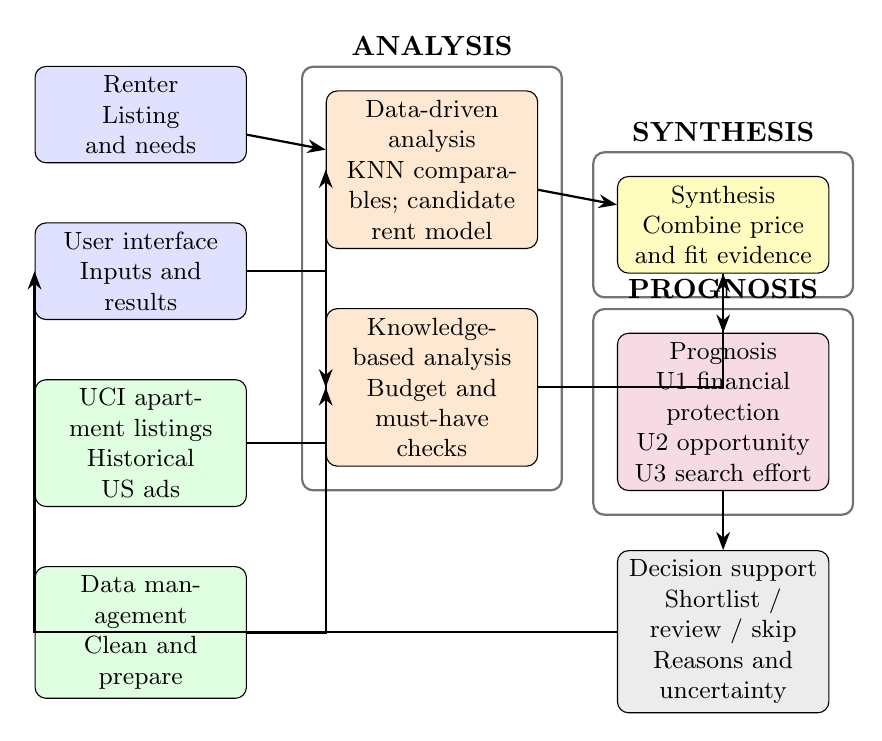
\begin{tikzpicture}[
  >=Stealth,
  node distance=0.75cm and 0.9cm,
  block/.style={
    draw,
    rounded corners,
    align=center,
    minimum width=2.65cm,
    minimum height=0.9cm,
    text width=2.45cm,
    font=\small
  },
  user/.style={block, fill=blue!12},
  data/.style={block, fill=green!12},
  analysis/.style={block, fill=orange!18},
  synthesis/.style={block, fill=yellow!25},
  prognosis/.style={block, fill=purple!14},
  output/.style={block, fill=gray!15},
  stage/.style={draw=black!55, rounded corners, thick, inner sep=0.3cm},
  flow/.style={->, thick}
]

% Three-column layout keeps the architecture readable at page width.
\node[user] (renter) {Renter\\Listing and needs};
\node[user, below=of renter] (interface) {User interface\\Inputs and results};
\node[data, below=of interface] (dataset) {UCI apartment listings\\Historical US ads};
\node[data, below=of dataset] (management) {Data management\\Clean and prepare};

% Analysis stage: data-driven comparisons and knowledge-based checks.
\node[analysis, right=1.0cm of renter, yshift=-0.7cm] (compare) {Data-driven analysis\\KNN comparables; candidate rent model};
\node[analysis, below=of compare] (constraints) {Knowledge-based analysis\\Budget and must-have checks};
\node[stage, fit=(compare)(constraints),
  label={[font=\bfseries]above:ANALYSIS}] (analysis-stage) {};

% Synthesis and prognosis lead to an explained recommendation.
\node[synthesis, right=1.0cm of compare, yshift=-0.7cm] (synth) {Synthesis\\Combine price and fit evidence};
\node[prognosis, below=of synth] (prognosis) {Prognosis\\U1 financial protection\\U2 opportunity\\U3 search effort};
\node[output, below=of prognosis] (recommendation) {Decision support\\Shortlist / review / skip\\Reasons and uncertainty};
\node[stage, fit=(synth),
  label={[font=\bfseries]above:SYNTHESIS}] (synthesis-stage) {};
\node[stage, fit=(prognosis),
  label={[font=\bfseries]above:PROGNOSIS}] (prognosis-stage) {};

% User and data inputs feed analysis; the recommendation returns to the renter.
\draw[flow] (renter) -- (compare);
\draw[flow] (interface.east) -| (constraints.west);
\draw[flow] (dataset.east) -| (compare.west);
\draw[flow] (management.east) -| (constraints.west);
\draw[flow] (compare) -- (synth);
\draw[flow] (constraints.east) -| (synth.south);
\draw[flow] (synth) -- (prognosis);
\draw[flow] (prognosis) -- (recommendation);
\draw[flow] (recommendation.west) -| (interface.west);

\end{tikzpicture}%
}
\caption{RentWise architecture mapped to the course's analysis, synthesis, and prognosis stages. Candidate methods are subject to validation.}
\label{fig:idss-architecture}
\end{figure}

\section{Modules and Information Flow}

The proposed prototype consists of the following modules, aligned with
Figure~\ref{fig:idss-architecture}:

\begin{enumerate}
  \item \textbf{User interface:} collects listing details and the renter's
  budget and housing preferences, then displays estimates, checks, and
  explanations.

  \item \textbf{Data management and preprocessing:} loads rental records,
  validates relevant fields, standardises units and categories, and
  prepares location and listing attributes for comparison and modelling.

  \item \textbf{Analysis modules:} the data-driven module retrieves
  comparable records using characteristics such as location, size,
  bedrooms, and bathrooms, and evaluates candidate regression models for
  reference asking-rent estimation. The knowledge-based module checks
  mandatory requirements. The actual model and evaluation results must
  be specified after the proposed methods have been tested.

  \item \textbf{Synthesis module:} keeps mandatory rule checks separate
  from optional preferences and combines them, potentially using a
  Weighted Sum Model, to form the shortlist, review, and skip alternatives.

  \item \textbf{Prognosis and explanation module:} assesses the price
  position, fit, and uncertainty associated with each alternative, then
  presents the recommendation and supporting reasons. It does not
  forecast landlord responses or application success.

  \item \textbf{User interface:} presents the evidence and recommendation
  so the renter can accept, refine, or reject the system's advice.
\end{enumerate}

Information flows from the renter's case and preferences, and from the
historical dataset, into the analysis stage. The data-driven and
knowledge-based analyses feed synthesis, which forms decision
alternatives. Prognosis assesses their price position, fit, and
uncertainty. The interface returns the recommendation and its evidence;
the renter makes the final decision. The repository currently documents
and implements data cleaning; the candidate recommendation models and
Streamlit interface remain proposed components until implemented and
evaluated.

\section{Software Tools and Technologies}

The repository uses Python 3.12 and the \texttt{uv} environment and
dependency manager. The current cleaning pipeline uses Pandas and NumPy
to prepare the UCI listing data. Scikit-learn is listed for candidate
similarity and predictive modelling, while Streamlit is listed for the
planned interface. These modelling and interface choices are proposals
to be confirmed through implementation and evaluation; no final model
algorithm or model performance is claimed in this chapter.

% ============================================================
% 4. DATA PREPROCESSING
% ============================================================
\chapter{Data Pre-processing Summary}
\label{ch:preprocessing}

\section{Data Sources}
[Describe each raw dataset or database: source, URL or access details, variables, number of records, time period, and license if relevant.]

\section{Data Understanding and Quality Assessment}
[Describe the exploratory analysis and quality issues found, such as missing values, duplicates, outliers, inconsistent formats, class imbalance, or noisy records.]

\section{Pre-processing Pipeline}
[Explain the operations applied, why they were needed, and the order in which they were performed.]

\begin{figure}[H]
\centering
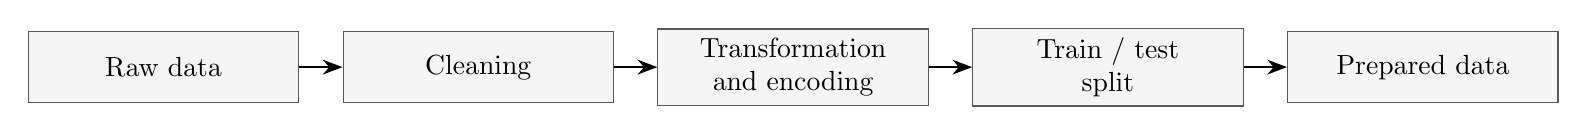
\begin{tikzpicture}[node distance=0.65cm and 0.55cm]
  \node[process] (raw) {Raw data};
  \node[process,right=of raw] (clean) {Cleaning};
  \node[process,right=of clean] (transform) {Transformation\\and encoding};
  \node[process,right=of transform] (split) {Train / test\\split};
  \node[process,right=of split] (ready) {Prepared data};
  \draw[arrow] (raw)--(clean);
  \draw[arrow] (clean)--(transform);
  \draw[arrow] (transform)--(split);
  \draw[arrow] (split)--(ready);
\end{tikzpicture}
\caption{Example data pre-processing pipeline. Adapt it to the actual workflow.}
\label{fig:preprocessing}
\end{figure}

\section{Final Dataset}
[Report the final dataset dimensions, selected features, target variable (if any), and any relevant changes after preprocessing.]

\begin{table}[H]
\centering
\caption{Summary of datasets before and after preprocessing.}
\label{tab:datasets}
\begin{tabularx}{\textwidth}{p{3cm} p{2cm} p{2cm} X}
\toprule
\textbf{Dataset} & \textbf{Records} & \textbf{Features} & \textbf{Notes}\\
\midrule
Raw & [N] & [N] & [Source / issues]\\
Preprocessed & [N] & [N] & [Cleaning / transformations]\\
Training & [N] & [N] & [Split details]\\
Testing & [N] & [N] & [Split details]\\
\bottomrule
\end{tabularx}
\end{table}

% ============================================================
% 5. DATA-DRIVEN MODELS
% ============================================================
\chapter{Data-driven IDSS Models}
\label{ch:datadriven}

\section{Modelling Objectives}
[Explain which decision-support tasks are addressed by data-driven modelling and why the selected approaches are appropriate.]

\section{Model 1: [Model name]}
\subsection{Method and Rationale}
[Describe the algorithm, its role in the IDSS, and why it was selected.]
\subsection{Inputs, Outputs, and Configuration}
[Specify features, target, important hyperparameters, and output format.]
\subsection{Training Procedure}
[Describe the training process, validation strategy, and software used.]
\subsection{Results}
[Present relevant results using tables or figures. Explain what the results mean for the decisions supported.]

\begin{table}[H]
\centering
\caption{Example model evaluation results. Replace metrics with those appropriate to your task.}
\label{tab:modelresults}
\begin{tabular}{lc}
\toprule
\textbf{Metric} & \textbf{Value}\\
\midrule
{[Metric 1]} & [Value]\\
{[Metric 2]} & [Value]\\
{[Metric 3]} & [Value]\\
\bottomrule
\end{tabular}
\end{table}

\section{Additional Models (if applicable)}
[Repeat the previous model structure for each additional model. Include descriptive, discriminant, predictive, or associative models as appropriate.]

\section{Model Output and Integration}
[Explain how trained models are represented and used at system runtime. For example, describe how a trained decision tree is converted into machine-readable rules and evaluated on new cases.]

% ============================================================
% 6. POSTPROCESSING AND VALIDATION
% ============================================================
\chapter{Data Post-processing and Model Validation}
\label{ch:validation}

\section{Post-processing}
[Describe how model outputs are transformed into useful information for users, including ranking, thresholds, aggregation, formatting, or explanation.]

\section{Validation Strategy}
[Describe the validation design, test data, baselines, metrics, and safeguards against data leakage.]

\section{Validation Results}
[Present the validation results and interpret them in relation to the intended decisions.]

\section{Limitations and Reliability}
[Discuss uncertainty, bias, generalizability, data limitations, and cases where recommendations should be reviewed by a human.]

% ============================================================
% 7. MODEL-DRIVEN TECHNIQUES
% ============================================================
\chapter{Model-driven IDSS Techniques}
\label{ch:modeldriven}

\section{Knowledge-based Component}
[Describe the expert knowledge, rules, ontology, constraints, or other knowledge representation used. Identify its source and how it was elicited or constructed.]

\section{Reasoning Mechanism}
[Explain how the system applies the knowledge: rule-based inference, case-based reasoning, qualitative reasoning, simulation, or another technique.]

\section{Example Rules or Knowledge Structures}
\begin{table}[H]
\centering
\caption{Example knowledge rules. Replace with rules actually used in the prototype.}
\label{tab:rules}
\begin{tabularx}{\textwidth}{p{1cm} X X}
\toprule
\textbf{ID} & \textbf{Condition (IF)} & \textbf{Conclusion / action (THEN)}\\
\midrule
R1 & [Condition] & [Conclusion]\\
R2 & [Condition] & [Conclusion]\\
R3 & [Condition] & [Conclusion]\\
\bottomrule
\end{tabularx}
\end{table}

\section{Interaction with Data-driven Models}
[Explain how the knowledge-based and data-driven components complement one another and contribute to the final decision support.]

% ============================================================
% 8. USE CASES
% ============================================================
\chapter{Testing Use Cases}
\label{ch:usecases}

[Describe at least three use cases that demonstrate how the IDSS supports different decision-making processes. Use realistic inputs and report the system outputs.]

\section{Use Case 1: [Name]}
\textbf{Goal:} [What decision is being supported?]\\
\textbf{Actor:} [Who uses the system?]\\
\textbf{Initial conditions:} [Relevant context.]\\
\textbf{Input data:} [Values or scenario.]\\
\textbf{Steps:}
\begin{enumerate}
  \item [Step 1]
  \item [Step 2]
  \item [Step 3]
\end{enumerate}
\textbf{Expected output:} [Expected recommendation or result.]\\
\textbf{Actual output:} [Observed system result.]\\
\textbf{Assessment:} [Did the system behave as expected? Explain.]

\section{Use Case 2: [Name]}
\textbf{Goal:} [Goal.]\\
\textbf{Actor:} [Actor.]\\
\textbf{Input data:} [Scenario and inputs.]\\
\textbf{Steps:}
\begin{enumerate}
  \item [Step 1]
  \item [Step 2]
  \item [Step 3]
\end{enumerate}
\textbf{Expected output:} [Expected result.]\\
\textbf{Actual output:} [Observed result.]\\
\textbf{Assessment:} [Evaluation.]

\section{Use Case 3: [Name]}
\textbf{Goal:} [Goal.]\\
\textbf{Actor:} [Actor.]\\
\textbf{Input data:} [Scenario and inputs.]\\
\textbf{Steps:}
\begin{enumerate}
  \item [Step 1]
  \item [Step 2]
  \item [Step 3]
\end{enumerate}
\textbf{Expected output:} [Expected result.]\\
\textbf{Actual output:} [Observed result.]\\
\textbf{Assessment:} [Evaluation.]

\section{Use Case Comparison}
\begin{table}[H]
\centering
\caption{Summary of the use cases tested.}
\label{tab:usecases}
\begin{tabularx}{\textwidth}{p{1.5cm} p{2.5cm} X X}
\toprule
\textbf{Use case} & \textbf{Decision} & \textbf{Main input} & \textbf{Outcome}\\
\midrule
UC1 & [Decision] & [Input] & [Outcome]\\
UC2 & [Decision] & [Input] & [Outcome]\\
UC3 & [Decision] & [Input] & [Outcome]\\
\bottomrule
\end{tabularx}
\end{table}

% ============================================================
% 9. GLOBAL EVALUATION
% ============================================================
\chapter{Global Evaluation of the IDSS and Conclusions}
\label{ch:evaluation}

\section{System Performance}
[Evaluate the prototype in the designed scenarios. Discuss functional correctness, response time, usability, quality of recommendations, and other relevant performance dimensions.]

\section{Achievement of Objectives}
[Review the objectives from \cref{ch:domain} and state which were achieved, partially achieved, or not achieved. Support the assessment with evidence.]

\section{Strengths and Limitations}
[Summarize the main strengths and current limitations of the complete IDSS.]

\section{Conclusions}
[Present the main conclusions from the development and evaluation of the prototype.]

% ============================================================
% 10. FUTURE WORK
% ============================================================
\chapter{Future Work and Improvements}
\label{ch:future}

[Describe realistic next steps. Consider data quality and quantity, additional models, knowledge acquisition, explainability, user experience, security, deployment, and evaluation with real users where relevant.]

\begin{itemize}[leftmargin=*]
  \item [Improvement 1 and its expected benefit.]
  \item [Improvement 2 and its expected benefit.]
  \item [Improvement 3 and its expected benefit.]
\end{itemize}

% ============================================================
% 11. PROJECT PLANNING / GANTT
% ============================================================
\chapter{Project Planning: Gantt Diagram}
\label{ch:gantt}

[Explain the project phases, milestones, dependencies, and how the work was planned. Adapt the dates and tasks below.]

\begin{figure}[H]
\centering
\begin{ganttchart}[
  hgrid,
  vgrid,
  x unit=0.85cm,
  y unit chart=0.65cm,
  title height=1,
  bar height=0.55,
  group height=0.6,
  title label font=\small,
  bar label font=\small,
  group label font=\small\bfseries
]{1}{10}
  \gantttitle{Project timeline (replace periods with actual dates)}{10}\\
  \gantttitlelist{1,...,10}{1}\\
  \ganttgroup{Planning and analysis}{1}{2}\\
  \ganttbar{Domain and decision definition}{1}{2}\\
  \ganttbar{Data collection}{2}{3}\\
  \ganttgroup{Design and development}{3}{7}\\
  \ganttbar{Architecture and preprocessing}{3}{4}\\
  \ganttbar{Model development}{4}{6}\\
  \ganttbar{Interface and integration}{6}{7}\\
  \ganttgroup{Evaluation and delivery}{8}{10}\\
  \ganttbar{Testing and use cases}{8}{9}\\
  \ganttbar{Report and presentation}{8}{10}\\
  \ganttbar{Demo and final delivery}{10}{10}
\end{ganttchart}
\caption{Illustrative Gantt diagram. Update the timeline to reflect the team's actual plan and execution.}
\label{fig:gantt}
\end{figure}

% ============================================================
% 12. TEAM ASSIGNMENT AND RESPONSIBILITIES
% ============================================================
\chapter{Tasks Assignment and Team Responsibilities}
\label{ch:teamwork}

[Describe how responsibilities were distributed, how the team coordinated work, and how integration and review were handled.]

\begin{longtable}{p{3.2cm} p{2.5cm} p{7cm}}
\caption{Task assignment and responsibilities.}\label{tab:responsibilities}\\
\toprule
\textbf{Team member} & \textbf{Role} & \textbf{Assigned tasks and responsibilities}\\
\midrule
\endfirsthead
\toprule
\textbf{Team member} & \textbf{Role} & \textbf{Assigned tasks and responsibilities}\\
\midrule
\endhead
{[Member 1]} & [Role] & [Tasks]\\
{[Member 2]} & [Role] & [Tasks]\\
{[Member 3]} & [Role] & [Tasks]\\
{[Member 4]} & [Role] & [Tasks]\\
{[Member 5, if applicable]} & [Role] & [Tasks]\\
\bottomrule
\end{longtable}

% ============================================================
% 13. TIME SHEET
% ============================================================
\chapter{Team Time Sheet}
\label{ch:timesheet}

[Record the hours devoted by each team member to each task. Ensure the totals are consistent with the team's accounting.]

\begin{longtable}{p{4.0cm} *{5}{>{\centering\arraybackslash}p{1.35cm}}}
\caption{Hours devoted by each team member to each task. Adapt the number of member columns to your team.}\label{tab:timesheet}\\
\toprule
\textbf{Task} & \textbf{M1} & \textbf{M2} & \textbf{M3} & \textbf{M4} & \textbf{M5}\\
\midrule
\endfirsthead
\toprule
\textbf{Task} & \textbf{M1} & \textbf{M2} & \textbf{M3} & \textbf{M4} & \textbf{M5}\\
\midrule
\endhead
Domain analysis & [h] & [h] & [h] & [h] & [h]\\
Data collection & [h] & [h] & [h] & [h] & [h]\\
Preprocessing & [h] & [h] & [h] & [h] & [h]\\
Model development & [h] & [h] & [h] & [h] & [h]\\
Knowledge component & [h] & [h] & [h] & [h] & [h]\\
Interface and integration & [h] & [h] & [h] & [h] & [h]\\
Testing and evaluation & [h] & [h] & [h] & [h] & [h]\\
Documentation and demo & [h] & [h] & [h] & [h] & [h]\\
\midrule
\textbf{Total hours} & [h] & [h] & [h] & [h] & [h]\\
\bottomrule
\end{longtable}

\section{Global Accounting per Team Member}
\begin{table}[H]
\centering
\caption{Total hours per team member.}
\label{tab:hours}
\begin{tabular}{lc}
\toprule
\textbf{Team member} & \textbf{Total hours}\\
\midrule
{[Member 1]} & [Hours]\\
{[Member 2]} & [Hours]\\
{[Member 3]} & [Hours]\\
{[Member 4]} & [Hours]\\
{[Member 5, if applicable]} & [Hours]\\
\bottomrule
\end{tabular}
\end{table}

% ============================================================
% REFERENCES
% ============================================================
\begin{thebibliography}{99}
\addcontentsline{toc}{chapter}{References}

\bibitem{uci_apartment_dataset}
UCI Machine Learning Repository.
\textit{Apartment for Rent Classified}. 2019.
doi: \href{https://doi.org/10.24432/C5X623}{10.24432/C5X623}.
Available at:
\url{https://archive.ics.uci.edu/dataset/555/apartment}.

\end{thebibliography}

% ============================================================
% APPENDICES
% ============================================================
\appendix
\chapter{Additional Figures and Tables}
[Add supplementary plots, detailed metrics, screenshots, or tables that support the report but are not essential to the main narrative.]

\chapter{Implementation Details}
[Add technical details, selected code excerpts, configuration information, or links to the project repository. Do not include large source files in the report; deliver source code in the required Source folder.]

\chapter{README and Deliverable Structure}
[Briefly describe the contents of the final ZIP package and how to run the prototype/demo.]

\end{document}
